\documentclass[11pt,a4paper]{article}

\usepackage[T1]{fontenc}
\usepackage[utf8]{inputenc}
\usepackage{mathpazo}
\linespread{1.06}
\usepackage[a4paper,margin=2.5cm]{geometry}
\usepackage{microtype}
\usepackage{amsmath}
\usepackage{graphicx}
\usepackage{booktabs}
\usepackage{longtable}
\usepackage{tabularx}
\usepackage{threeparttable}
\usepackage[table]{xcolor}
\usepackage{caption}
\captionsetup{font=small,labelfont=bf,labelsep=period}
\usepackage{enumitem}
\setlist{itemsep=2pt,topsep=4pt}
\usepackage[numbers,sort&compress]{natbib}
\usepackage[hidelinks]{hyperref}
\usepackage[capitalise,noabbrev]{cleveref}
\usepackage{url}
\usepackage[section]{placeins}
\urlstyle{same}

% Generated by make_stats.py from the SDG Explorer India data. Do not edit by hand.
\newcommand{\nRecords}{58{,}658}
\newcommand{\nObs}{51{,}700}
\newcommand{\nNumeric}{51{,}695}
\newcommand{\nText}{5}
\newcommand{\nNA}{6{,}958}
\newcommand{\nIndicators}{301}
\newcommand{\nSeries}{751}
\newcommand{\yFirst}{1977}
\newcommand{\yLast}{2026}
\newcommand{\nBeforeFifteen}{5{,}285}
\newcommand{\obsUN}{12{,}469}
\newcommand{\recUN}{13{,}413}
\newcommand{\naUN}{944}
\newcommand{\indUN}{212}
\newcommand{\serUN}{493}
\newcommand{\firstUN}{1977}
\newcommand{\lastUN}{2026}
\newcommand{\preUN}{5{,}255}
\newcommand{\obsMospi}{1{,}834}
\newcommand{\recMospi}{1{,}886}
\newcommand{\naMospi}{52}
\newcommand{\indMospi}{224}
\newcommand{\serMospi}{224}
\newcommand{\firstMospi}{2011}
\newcommand{\lastMospi}{2025}
\newcommand{\preMospi}{30}
\newcommand{\obsNfhs}{37{,}397}
\newcommand{\recNfhs}{43{,}359}
\newcommand{\naNfhs}{5{,}962}
\newcommand{\indNfhs}{13}
\newcommand{\serNfhs}{34}
\newcommand{\firstNfhs}{2015}
\newcommand{\lastNfhs}{2019}
\newcommand{\preNfhs}{0}
\newcommand{\numMospi}{1{,}829}
\newcommand{\textMospi}{5}
\newcommand{\obsNational}{14{,}303}
\newcommand{\unPages}{15}
\newcommand{\unApiRecords}{14{,}594}
\newcommand{\unRepeats}{1{,}181}
\newcommand{\unUnique}{13{,}413}
\newcommand{\moSnapshot}{277}
\newcommand{\moParsed}{224}
\newcommand{\moNotParsed}{53}
\newcommand{\moRows}{1{,}886}
\newcommand{\moRowsChecked}{1{,}303}
\newcommand{\moConfirmedWords}{1{,}302}
\newcommand{\moConfirmedVisual}{1}
\newcommand{\moGridTables}{23}
\newcommand{\moGridValues}{392}
\newcommand{\moPdfCreated}{2025-06-27}
\newcommand{\dateUN}{2026-10-15}
\newcommand{\shaUN}{7a8c01811b39}
\newcommand{\dateMospi}{2026-10-15}
\newcommand{\shaMospi}{9f7623adfc13}
\newcommand{\mbMospi}{37.1}
\newcommand{\dateNiti}{2026-10-15}
\newcommand{\shaNiti}{a8b3dab605b6}
\newcommand{\mbNiti}{23.9}
\newcommand{\dateMpi}{2026-10-21}
\newcommand{\shaMpi}{4c694f54b919}
\newcommand{\mbMpi}{22.7}
\newcommand{\dateAsp}{2026-10-21}
\newcommand{\shaAsp}{24fee1772b16}
\newcommand{\mbAsp}{0.5}
\newcommand{\dateGeo}{2026-10-15}
\newcommand{\shaGeo}{b61ebc11a748}
\newcommand{\mbGeo}{17.1}
\newcommand{\unDiscontinued}{15}
\newcommand{\unListed}{1{,}047}
\newcommand{\unListedInd}{251}
\newcommand{\unWithNum}{493}
\newcommand{\unOnlyNA}{12}
\newcommand{\unNoRecord}{542}
\newcommand{\unShare}{47.1}
\newcommand{\bestGoal}{7}
\newcommand{\bestGoalName}{Affordable and Clean Energy}
\newcommand{\bestGoalShare}{100}
\newcommand{\worstGoal}{4}
\newcommand{\worstGoalName}{Quality Education}
\newcommand{\worstGoalShare}{25}
\newcommand{\nGoalsBelowHalf}{9}
\newcommand{\goalsBelowHalf}{4, 6, 8, 10, 11, 13, 14, 16, 17}
\newcommand{\unLatestMedian}{2023}
\newcommand{\unLatestSinceTwenty}{443}
\newcommand{\unLatestSinceTwentyPct}{90}
\newcommand{\unLatestSinceTwentyTwo}{379}
\newcommand{\unLatestSinceTwentyTwoPct}{77}
\newcommand{\unOldest}{2007}
\newcommand{\unYearsMedian}{7}
\newcommand{\unSingleYear}{82}
\newcommand{\unSingleYearPct}{17}
\newcommand{\moYearsMedian}{7}
\newcommand{\moFewYears}{48}
\newcommand{\moFewYearsPct}{22}
\newcommand{\natFewYears}{168}
\newcommand{\natSeriesTotal}{716}
\newcommand{\natFewYearsPct}{23}
\newcommand{\cityObs}{371}
\newcommand{\cityN}{91}
\newcommand{\citySeries}{6}
\newcommand{\nitiN}{36}
\newcommand{\nitiMax}{79}
\newcommand{\nitiMin}{57}
\newcommand{\nitiTop}{Kerala and Uttarakhand}
\newcommand{\nitiBottom}{Bihar}
\newcommand{\nitiFront}{32}
\newcommand{\nitiPerformer}{4}
\newcommand{\indiaA}{57}
\newcommand{\indiaB}{60}
\newcommand{\indiaC}{66}
\newcommand{\indiaD}{71}
\newcommand{\nitiGoalScores}{15}
\newcommand{\indiaGoalMax}{7}
\newcommand{\indiaGoalMaxScore}{96}
\newcommand{\indiaGoalMin}{5}
\newcommand{\indiaGoalMinScore}{49}
\newcommand{\nitiRows}{98}
\newcommand{\nDistricts}{704}
\newcommand{\nDistStates}{34}
\newcommand{\nNfhsSeries}{34}
\newcommand{\nNfhsGoals}{8}
\newcommand{\nBracket}{1{,}806}
\newcommand{\nfhsSheets}{704}
\newcommand{\nfhsRenumbered}{2}
\newcommand{\nfhsSkippedCells}{13}
\newcommand{\nfhsSkippedSheets}{9}
\newcommand{\pvShared}{17{,}661}
\newcommand{\pvSame}{17{,}658}
\newcommand{\pvDiff}{3}
\newcommand{\pvDistricts}{340}
\newcommand{\pvTheirDistricts}{341}
\newcommand{\pvDiffDistricts}{Dhule}
\newcommand{\mpiRows}{709}
\newcommand{\mpiStray}{3}
\newcommand{\mpiMatched}{704}
\newcommand{\mpiAliases}{57}
\newcommand{\mpiUnmatched}{5}
\newcommand{\hMedFive}{12.50}
\newcommand{\hOtherBoundary}{63}
\newcommand{\hPairN}{572}
\newcommand{\hMedFourPair}{23.72}
\newcommand{\hMedFivePair}{12.93}
\newcommand{\hDeclined}{552}
\newcommand{\hRose}{20}
\newcommand{\hSame}{0}
\newcommand{\bandOneLo}{0.00}
\newcommand{\bandOneHi}{4.13}
\newcommand{\bandOneN}{140}
\newcommand{\bandTwoLo}{4.24}
\newcommand{\bandTwoHi}{8.74}
\newcommand{\bandTwoN}{141}
\newcommand{\bandThreeLo}{8.77}
\newcommand{\bandThreeHi}{15.45}
\newcommand{\bandThreeN}{141}
\newcommand{\bandFourLo}{15.57}
\newcommand{\bandFourHi}{23.14}
\newcommand{\bandFourN}{141}
\newcommand{\bandFiveLo}{23.16}
\newcommand{\bandFiveHi}{54.44}
\newcommand{\bandFiveN}{141}
\newcommand{\hMaxDistrict}{Bahraich}
\newcommand{\hMaxState}{Uttar Pradesh}
\newcommand{\hMax}{54.44}
\newcommand{\hMin}{0.00}
\newcommand{\hMinN}{1}
\newcommand{\aspListed}{112}
\newcommand{\aspMatched}{108}
\newcommand{\aspMedH}{26.72}
\newcommand{\othMedH}{10.09}
\newcommand{\othN}{596}
\newcommand{\aspInPoorest}{63}
\newcommand{\aspInTopTwo}{84}
\newcommand{\aspInLeastPoor}{4}
\newcommand{\aspAUC}{0.80}
\newcommand{\nIndAssoc}{34}
\newcommand{\nComp}{9}
\newcommand{\rhoCompMin}{0.20}
\newcommand{\rhoCompMax}{0.77}
\newcommand{\otherTopOne}{institutional births}
\newcommand{\otherTopOneRho}{\ensuremath{-}0.75}
\newcommand{\otherTopTwo}{women (15-49) who are literate}
\newcommand{\otherTopTwoRho}{\ensuremath{-}0.73}
\newcommand{\otherTopThree}{deaths in the last 3 years registered}
\newcommand{\otherTopThreeRho}{\ensuremath{-}0.69}
\newcommand{\nWeak}{5}
\newcommand{\nStrongAll}{15}
\newcommand{\unPeakYear}{2020}
\newcommand{\unPeakN}{326}
\newcommand{\buildDate}{2026-10-26}
\newcommand{\pctOutside}{116}
\newcommand{\pctOutsideSeries}{19}
\newcommand{\valErrors}{0}
\newcommand{\unRelease}{2026.Q3.G.01}
\newcommand{\nTests}{84}
\newcommand{\nTestFiles}{8}


\definecolor{ink}{HTML}{1B2140}
\makeatletter\newcommand{\inputtab}[1]{\@@input #1 }\makeatother
\newcommand{\code}[1]{\texttt{\small #1}}

\title{\textbf{SDG Explorer India: a verified open pipeline and interactive atlas of official Sustainable Development Goal data for India, from national series to 704 districts}}
\author{Sahil\\[2pt]
\small Whiting School of Engineering, Johns Hopkins University, Baltimore, MD, USA\\
\small \href{mailto:sfnu1@jh.edu}{sfnu1@jh.edu}}
\date{\small October 2026\quad$\cdot$\quad Data build \buildDate}

\begin{document}
\maketitle

\begin{abstract}
\noindent
Official data on India's progress towards the Sustainable Development Goals (SDGs) are published by several agencies in formats ranging from an application programming interface to scanned reports, which makes them hard to combine, check and reuse. SDG Explorer India is an open, tested Python pipeline and a static website that assemble four official observation sources---the UN Global SDG Indicators Database, the Ministry of Statistics and Programme Implementation's National Indicator Framework Progress Report 2025, the National Family Health Survey (NFHS) district fact sheets, and NITI Aayog's SDG India Index 2023--24---together with two district-level grouping sources from NITI Aayog: the district tables of the National Multidimensional Poverty Index 2023 and the list of 112 Aspirational Districts. The current build holds \nObs{} published values (\nNumeric{} numeric and \nText{} text values) for \nIndicators{} indicator codes and \nSeries{} data series across all 17 goals, for India and \nDistricts{} districts, with observation years from \yFirst{} to \yLast{}; a further \nNA{} records are the publishers' own ``not available'' markers. Every value is kept as published and traced to its source file by URL and SHA-256 checksum, and each source passes an independent check, such as a second PDF reader, an arithmetic identity or comparison with an independent digitisation. The assembled data show that only \unWithNum{} of the \unListed{} series in the UN global indicator list (\unShare\%) have at least one numeric value for India. Across districts, the multidimensional poverty headcount ratio fell between NFHS-4 and NFHS-5 in \hDeclined{} of \hPairN{} districts with both estimates, and it is strongly associated with indicators of institutional delivery, women's literacy and civil registration. The data, code and website are openly available.
\end{abstract}

\noindent\textbf{Keywords:} Sustainable Development Goals; India; official statistics; data provenance; PDF table extraction; multidimensional poverty; district data; open data

% =====================================================================
\section{Introduction}

The 2030 Agenda for Sustainable Development sets 17 goals and 169 targets \citep{un2015agenda}, monitored through a global indicator framework adopted by the UN General Assembly \citep{un2017framework}. For India, the relevant official numbers are spread across several publishers. The UN Statistics Division maintains the Global SDG Indicators Database and an API \citep{unsd_sdgdb}; the Ministry of Statistics and Programme Implementation (MoSPI) publishes the National Indicator Framework (NIF) progress report as a PDF report \citep{mospi2025nif}; NITI Aayog publishes the SDG India Index, a composite score for States and Union Territories \citep{niti2024sdgii}; and the National Family Health Survey (NFHS) publishes district estimates as one PDF fact sheet per district \citep{iips2021nfhs5,nfhs5_dfs}.

These sources differ in format, coverage, units, and in how they mark missing values. Combining them by hand is slow and error-prone, and the gaps in the data---goals and districts with few or no values---are easy to miss when only the available numbers are shown. SDG Explorer India \citep{sdgexplorer} was built to address three needs:
\begin{enumerate}[label=(\roman*)]
  \item a single, reproducible table of every official value for India, with its source file, page and checksum, in which nothing is imputed and missing values stay missing;
  \item explicit verification of each source, so that values read from PDFs can be trusted to the same degree as values read from an API;
  \item a website that makes both the data and their gaps visible to non-specialists, including a district view that supports careful comparison.
\end{enumerate}
This paper describes the sources (\cref{sec:sources}), the pipeline and its verification (\cref{sec:methods,sec:validation}), the resulting data (\cref{sec:records}), descriptive analyses that the data support (\cref{sec:analysis}), the website (\cref{sec:web}), and the limitations (\cref{sec:limits}). All numbers in this paper are generated from the project's processed data files by a script, so the text and the data cannot drift apart.

% =====================================================================
\section{Sources}\label{sec:sources}

\Cref{tab:sources} lists the sources. They are grouped by how their numbers may be used. \emph{Observations} are published indicator values. \emph{Composite index} scores (NITI Aayog's SDG India Index) are built by the publisher from normalised, weighted indicators; they are stored separately and never mixed with observations. \emph{District grouping} sources describe districts (poverty level, programme membership) and are used only to filter and group districts.

\begin{table}[!htbp]
\centering
\small
\caption{Sources used in the current build. Retrieval dates and SHA-256 prefixes are from the provenance record stored next to each raw file.}\label{tab:sources}
\begin{tabularx}{\textwidth}{>{\raggedright\arraybackslash}p{4.3cm} >{\raggedright\arraybackslash}p{2.2cm} >{\raggedright\arraybackslash}X >{\raggedright\arraybackslash}p{2.7cm}}
\toprule
Source & Kind & Geography and content & Retrieved (SHA-256) \\
\midrule
UN Global SDG Indicators Database, SDG API v1 \citep{unsd_sdgdb} & Observations & India, national; all series in the global indicator list (release \unRelease) & \dateUN{} (page 1: \code{\shaUN}) \\
MoSPI, NIF Progress Report 2025 \citep{mospi2025nif} & Observations & India, national; NIF ``Data Snapshot'' tables, \mbMospi{} MB PDF & \dateMospi{} (\code{\shaMospi}) \\
MoHFW/IIPS, NFHS-5 District Fact Sheets \citep{nfhs5_dfs} & Observations & \nDistricts{} districts; NFHS-5 (2019--21) and NFHS-4 (2015--16) columns & see \cref{sec:nfhs} \\
NITI Aayog, SDG India Index 2023--24 \citep{niti2024sdgii} & Composite index & 36 States/UTs and India; \mbNiti{} MB PDF & \dateNiti{} (\code{\shaNiti}) \\
NITI Aayog, National MPI: A Progress Review 2023 \citep{niti2023mpi} & District grouping & District headcount ratio, intensity and MPI, NFHS-4 and NFHS-5; \mbMpi{} MB PDF & \dateMpi{} (\code{\shaMpi}) \\
NITI Aayog, List of 112 Aspirational Districts \citep{niti_adp} & District grouping & 112 districts & \dateAsp{} (\code{\shaAsp}) \\
DataMeet, State boundaries \citep{datameet_maps} & Reference & 36 States/UTs (map only) & \dateGeo{} (\code{\shaGeo}) \\
\bottomrule
\end{tabularx}
\end{table}

% =====================================================================
\section{Methods}\label{sec:methods}

\subsection{Pipeline and provenance}
The pipeline is a Python package run from the command line: \code{fetch} downloads every source with retries and exponential back-off; \code{import} accepts files downloaded elsewhere; \code{build} parses the raw files, validates the result and writes the processed tables; \code{site} exports compact JSON for the website; and \code{report} prints the coverage manifest (\code{all} runs \code{fetch} and \code{build} together). Each raw file is stored unchanged next to a provenance record giving its URL, retrieval time, size and SHA-256 checksum. Every processed value carries the URL, raw file name and checksum of its source and, where applicable, the report page. A build that fails validation stops and leaves the previous build in place.

Large PDFs (the MoSPI, NITI and NFHS files) are not committed to the repository. Instead, the verified extracts made from them are committed under \code{data/reference/}, each tagged with the checksum of the PDF it was read from, so the processed data can be rebuilt without the PDFs; when a PDF is present and its checksum differs, the extract is rebuilt from it.

\subsection{Data rules}
Five rules apply to every source:
(1)~nothing is invented, imputed or interpolated, and missing years stay missing;
(2)~values are kept exactly as published, and values published as text (for example \code{<0.1}) remain text;
(3)~composite index scores are kept apart from observations;
(4)~observation years are kept separate from publication dates;
(5)~UN and MoSPI series for the same indicator code stay separate, because MoSPI's NIF codes are national indicators that follow the global target numbering but are not the same indicators.

\subsection{UN Global SDG Indicators Database}
All records for India (M49 area code 356) were requested in pages of 1{,}000. The API reported \unApiRecords{} records, and all \unPages{} pages were received; the build stops if any page is missing or the record count does not match the API's total. \unRepeats{} records were exact repeats: a series filed under several indicators is returned once per indicator. These copies were merged only after checking that their content was identical, leaving \unUnique{} records. Of these, \naUN{} are the UN's own ``NaN = Not Available'' markers, kept for the analysis of missing data but not counted as observations, which leaves \obsUN{} observations in \serUN{} series. Breakdowns (sex, age, location, cities and others) are kept as published.

\subsection{MoSPI NIF Progress Report 2025}
The report's Data Snapshot lists \moSnapshot{} national indicators. A table was parsed only when every row and column could be read without ambiguity; \moParsed{} indicators were parsed and \moNotParsed{} were listed with a reason and report page instead (\cref{tab:mospi}). Every one of the \moRowsChecked{} parsed table rows was checked by a second, independent method: the period and its values had to appear together on the printed page, using pdfplumber's word positions \citep{pdfplumber}. \moConfirmedWords{} rows passed; one value is a word that pdfplumber cannot extract and was confirmed on the rendered page image. A further \moGridTables{} tables with multi-line headers or grouping columns were read from their drawn gridlines (\moGridValues{} values), with column labels reviewed on the page images and every row confirmed against Poppler's text layout \citep{poppler}. The result is \moRows{} records, of which \numMospi{} are numeric, \textMospi{} are published as text and \naMospi{} are not-available markers.

\begin{table}[!htbp]
\centering\small
\caption{MoSPI NIF indicators not turned into data, by reason. Each is listed with its report page in the processed data.}\label{tab:mospi}
\begin{tabularx}{0.85\textwidth}{>{\raggedright\arraybackslash}X r}
\toprule
Reason & Indicators \\
\midrule
\inputtab{tab_mospi_np.tex}
\midrule
Total & \moNotParsed \\
\bottomrule
\end{tabularx}
\end{table}

\subsection{NFHS district fact sheets}\label{sec:nfhs}
Each of the \nfhsSheets{} district fact sheets lists 104 numbered key indicators with an NFHS-5 and, for districts that existed in 2015--16, an NFHS-4 column. The pipeline loads the \nNfhsSeries{} indicators that have a clear SDG counterpart, each labelled as the \emph{same} measure as a national NIF indicator or only \emph{related} to an SDG target. Indicators were matched by name, not only by printed number, because \nfhsRenumbered{} official sheets skip a number in their list. Values printed in brackets, which are based on 25--49 unweighted cases, are kept with a note (\nBracket{} values); ``na'' and ``*'' are kept as not-available markers. \nfhsSkippedCells{} indicator values in \nfhsSkippedSheets{} sheets, whose numbers are split across lines out of column order, were left out and listed. NFHS-5 published 707 district fact sheets; three of them (Chandigarh, Lakshadweep and Vidisha) are not in the public mirror from which the 704 PDFs were obtained, so those districts are absent from this build. The mirror was used because the official site was not reachable from the build machine; the checksums of the 704 files have not yet been compared with copies downloaded directly from the official site.

The result was compared with an independent digitisation of the same fact sheets \citep{pratap_nfhs5}, which covers \pvTheirDistricts{} districts. Matching on State, district name, indicator number and survey round gave \pvShared{} shared numeric values in \pvDistricts{} districts, of which \pvSame{} are identical. The \pvDiff{} differences are all in one district (\pvDiffDistricts) and involve three adjacent tobacco and alcohol indicators: the independent copy has the same numbers one row lower (for example, 38.2 appears there as women's alcohol use and here as men's tobacco use), which is consistent with a row shift in that copy.

\subsection{SDG India Index 2023--24}
The index report is a scanned document of low resolution, so its scores were read from the page images rather than by optical character recognition, and cross-checked against figures stated in the report text (for example, the range of State scores). The \nitiRows{} published scores are 36 State/UT composite scores for 2023--24, India's composite score for four editions (2018, 2019--20, 2020--21 and 2023--24), and India's goal scores. The ``change since 2020--21'' labels in the report were not legible at its resolution and are not included.

\subsection{National Multidimensional Poverty Index 2023: district tables}
NITI Aayog's national MPI follows the Alkire--Foster method \citep{alkire2011counting} with three equally weighted dimensions (health, education and standard of living) and 12 indicators; a person is multidimensionally poor when their weighted deprivation score is 33.33\% or more \citep{niti2023mpi}. For each State and UT the report prints a table of districts with, for both NFHS rounds, the headcount ratio $H$ (the percentage of people who are multidimensionally poor), the intensity $A$ (the average deprivation share among the poor) and $\mathrm{MPI} = H \times A$.

Some pages of the report carry an invisible copy of a neighbouring State's table beneath the printed one; for example, Assam's districts lie under Bihar's table. The copy is covered by white row rectangles drawn later, so it does not appear on the printed page, but it remains in the text layer and corrupts a naive extraction (it produces district names such as ``Aurangabad Biswanath''). The parser therefore drops every glyph whose box is entirely covered by filled shapes drawn after it, testing nine sample points per glyph because a glyph can straddle two row rectangles. Table columns are found from the numbers themselves, and a row is loaded only if it satisfies the identity $\mathrm{MPI} = H \times A$ within rounding ($|HA - \mathrm{MPI}| \le 0.0015$, with $H$ and $A$ as proportions). The parser read \mpiRows{} district rows; \mpiStray{} further rows of stray dashes with no district name and no values, remnants of the hidden layer, were listed and not loaded. As a second check, Poppler's text layout shows the same six values on one line for every row outside the Bihar page; Bihar's 38 rows, where Poppler mixes in the hidden copy, were compared one by one with the rendered page image.

\subsection{Aspirational Districts and district matching}
The list of Aspirational Districts was read from its table, and the serial numbers were required to run from 1 to 112. District names in the MPI tables and the Aspirational list were matched to the NFHS districts within the same State by exact name, then by a name in brackets, then by a reviewed alias table of \mpiAliases{} entries (spelling differences and renamings such as Gurugram/Gurgaon or the 2021 renaming of Sikkim's districts). A district that was split, merged or created after NFHS-5 is never assigned another district's value: all \nDistricts{} NFHS districts received an MPI row, and the \mpiUnmatched{} unmatched MPI rows (two undivided districts with NFHS-4 values only, one district absent from the fact-sheet set, and the single-district UTs of Chandigarh and Lakshadweep) are listed. Of the \aspListed{} Aspirational Districts, \aspMatched{} were linked; four were created after NFHS-5 or are absent from the fact sheets and are listed.

\subsection{Statistics}
District-level associations are described with Spearman's rank correlation $\rho$ \citep{spearman1904}, with 95\% confidence intervals from the Fisher transformation using the Bonett--Wright standard error $\sqrt{(1+\rho^2/2)/(n-3)}$ \citep{bonett2000}. Group differences are summarised by medians and, for two groups, by the Mann--Whitney probability that a randomly chosen district from one group has a higher value than one from the other \citep{mann1947}. No population weights are used: the unit is the district.

% =====================================================================
\section{Data records}\label{sec:records}

The processed data consist of an observations table (\nRecords{} records), an indicator and series list from the UN, a coverage table, the NITI index scores, a district context table, a geography register, a source register, a list of everything not parsed, and a build manifest. \Cref{tab:totals} summarises the observations.

\begin{table}[!htbp]
\centering\small
\caption{Observations by source in the current build. ``Observations'' exclude the publishers' not-available (N/A) markers.}\label{tab:totals}
\setlength{\tabcolsep}{4.5pt}
\begin{tabular}{lrrrrrc}
\toprule
Source & Records & N/A & Observations & Indicators & Series & Years \\
\midrule
UN SDG database & \recUN & \naUN & \obsUN & \indUN & \serUN & \firstUN--\lastUN \\
MoSPI NIF report 2025 & \recMospi & \naMospi & \obsMospi & \indMospi & \serMospi & \firstMospi--\lastMospi \\
NFHS fact sheets & \recNfhs & \naNfhs & \obsNfhs & \indNfhs & \serNfhs & NFHS-4, NFHS-5 \\
\midrule
All & \nRecords & \nNA & \nObs & \nIndicators & \nSeries & \yFirst--\yLast \\
\bottomrule
\end{tabular}
\par\smallskip\parbox{0.92\textwidth}{\footnotesize Indicators are counted as distinct full indicator codes (goal.target.number); a code used by two sources is counted once, although UN and NIF indicators with the same code are not always the same measure. NFHS indicators linked only to an SDG target, not to a numbered indicator, are not counted. NFHS observation years are the first year of each survey round (2015 and 2019). \nBeforeFifteen{} observations refer to years before 2015.}
\end{table}

\subsection{Coverage of the UN global indicator list}
The UN list used here contains \unListed{} series under \unListedInd{} indicators; each series is counted once, and \unDiscontinued{} series that every UN listing marks ``Not In Use'' are left out. Only \unWithNum{} of these series (\unShare\%) have at least one numeric value for India; \unOnlyNA{} have only not-available markers and \unNoRecord{} have no India record at all. Coverage differs widely by goal (\cref{fig:uncov,tab:goals}): it is highest for Goal~\bestGoal{} (\bestGoalName, \bestGoalShare\%) and lowest for Goal~\worstGoal{} (\worstGoalName, \worstGoalShare\%), and fewer than half the series have India data for \nGoalsBelowHalf{} of the 17 goals (Goals \goalsBelowHalf).

\begin{figure}[!htbp]
\centering
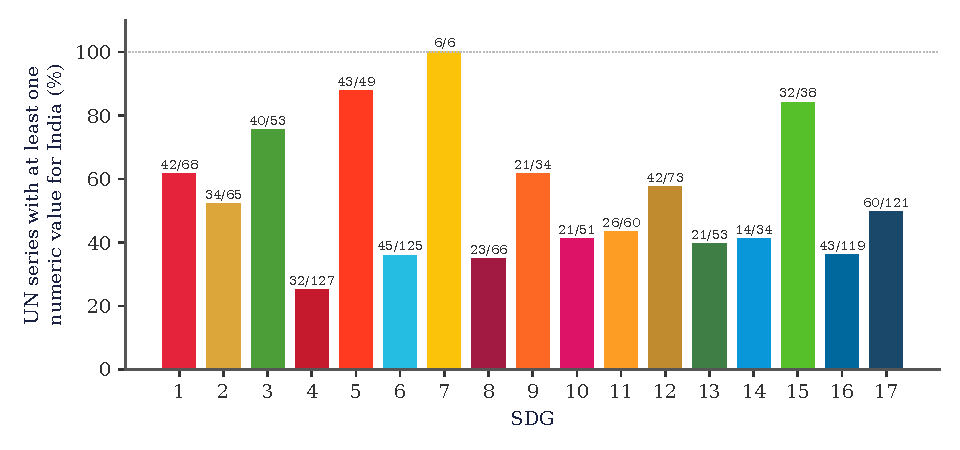
\includegraphics[width=0.92\textwidth]{fig_un_coverage.pdf}
\caption{Share of series in the UN global indicator list with at least one numeric value for India, by goal. Labels give series with data over series listed. A series linked to several goals is counted under each.}\label{fig:uncov}
\end{figure}

\begin{table}[!htbp]
\centering\small
\caption{National coverage by goal. \emph{UN listed}: series in the UN list; \emph{With data}: of these, series with at least one numeric value for India; \emph{MoSPI}: MoSPI NIF series with values; \emph{Values}: national numeric values from both sources; \emph{Years}: first and last observation year.}\label{tab:goals}
\setlength{\tabcolsep}{4pt}
\begin{tabular}{r>{\raggedright\arraybackslash}p{5.2cm}rrrrrc}
\toprule
Goal & Name & UN listed & With data & \% & MoSPI & Values & Years \\
\midrule
\inputtab{tab_goals.tex}
\bottomrule
\end{tabular}
\end{table}

\subsection{Time coverage and timeliness}
\Cref{fig:years} shows how many series have a value in each year. UN coverage rises from about 2000, peaks in \unPeakYear{} (\unPeakN{} series), and falls in the most recent years, which most likely reflects the lag between a reference year and the publication of its data rather than a fall in monitoring. The median UN series has values for \unYearsMedian{} distinct years, and its latest value refers to \unLatestMedian; \unLatestSinceTwentyTwo{} UN series (\unLatestSinceTwentyTwoPct\%) have a value for 2022 or later. \unSingleYear{} UN series (\unSingleYearPct\%) have a value for a single year only. Across both national sources, \natFewYears{} of \natSeriesTotal{} series (\natFewYearsPct\%) have values for fewer than three years, too few to describe a trend; the website shows such series as tables rather than charts (\cref{sec:web}). City breakdowns are available for \cityN{} cities in \citySeries{} urban series (\cityObs{} observations).

\begin{figure}[!htbp]
\centering
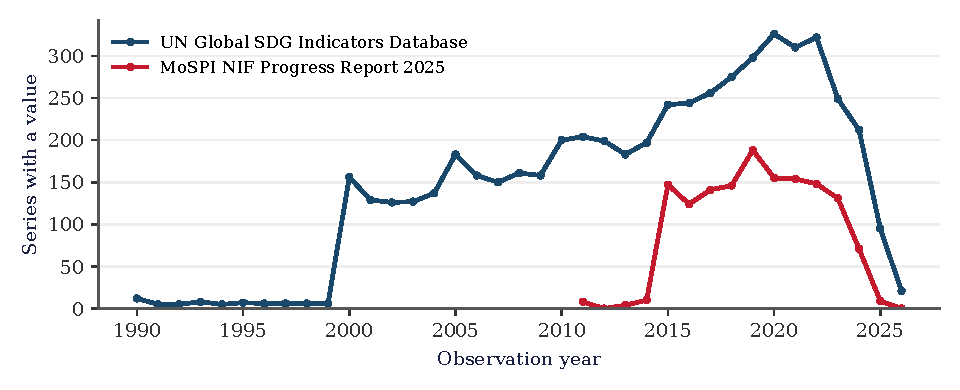
\includegraphics[width=0.92\textwidth]{fig_years.pdf}
\caption{Number of national series with at least one numeric value in each observation year, 1990 onwards, by source.}\label{fig:years}
\end{figure}

% =====================================================================
\section{Technical validation}\label{sec:validation}

Besides the source-specific checks in \cref{sec:methods}, every build runs a validation step that stops on any error. It requires the full schema; non-empty identifiers, source URLs and checksums; unique observation identifiers; goal numbers from 1 to 17; plausible years; known geographies; no composite index source in the observation table; index scores between 0 and 100; and that every missing number is explained by a published text value or not-available marker. The current build has \valErrors{} errors. One warning flags \pctOutside{} values in percentage units that fall outside 0--100, in \pctOutsideSeries{} UN series. Most are growth rates, changes or balances that can be negative, or ratios that can exceed 100 (such as expenditure against the approved budget, or tariff averages); they are kept as published. The repository contains \nTests{} automated tests in \nTestFiles{} files, run on every change by continuous integration. They include tests that:
\begin{itemize}
  \item trace 300 randomly sampled processed UN values back to the raw API files;
  \item check that the website holds exactly one entry for each processed national observation and goal, and that 400 sampled national and 300 sampled district values on the website equal their processed values;
  \item check that every MPI row satisfies $\mathrm{MPI} = H \times A$, that every alias points to an existing district, that matching is one-to-one, and, when the report PDF is present, that Poppler confirms each row;
  \item check that the Aspirational list has serial numbers 1 to 112;
  \item run the parsers on synthetic inputs that reproduce known difficulties (missing pages, renumbered fact sheets, values split across lines), so that the error handling is itself tested.
\end{itemize}
Tests that need the large PDFs are skipped when these are not present.

% =====================================================================
\section{Descriptive analyses}\label{sec:analysis}

This section reports what the assembled data show. The analyses are descriptive; they are not causal estimates.

\subsection{States and Union Territories: SDG India Index 2023--24}
NITI Aayog's composite scores for the \nitiN{} States and UTs range from \nitiMin{} (\nitiBottom) to \nitiMax{} (\nitiTop) (\cref{fig:niti}). In NITI Aayog's classification (Performer 50--64, Front Runner 65--99), \nitiFront{} States/UTs are Front Runners and \nitiPerformer{} are Performers. India's composite score rose from \indiaA{} in 2018 to \indiaB{} in 2019--20, \indiaC{} in 2020--21 and \indiaD{} in 2023--24; because NITI Aayog changed the indicator set between editions, these differences are not a pure trend. Among India's goal scores in 2023--24 (\nitiGoalScores{} goals are scored), the highest is for Goal~\indiaGoalMax{} (\indiaGoalMaxScore) and the lowest for Goal~\indiaGoalMin{} (\indiaGoalMinScore).

\begin{figure}[!htbp]
\centering
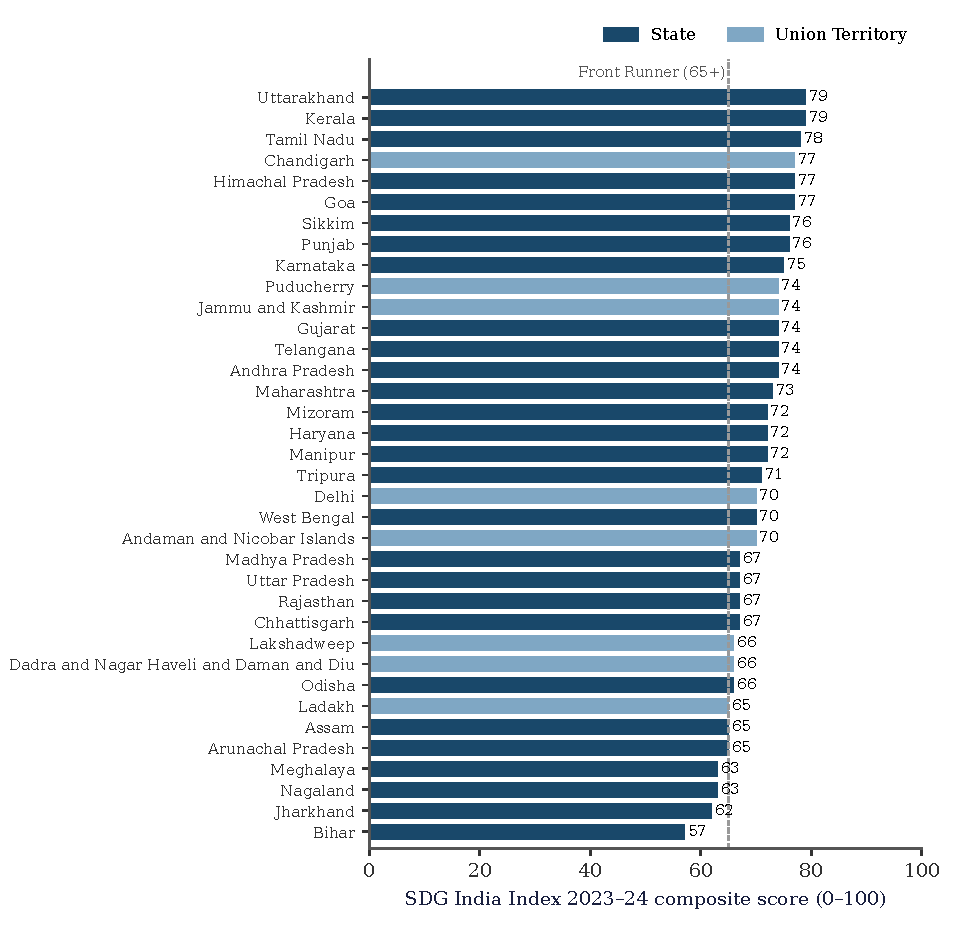
\includegraphics[width=0.78\textwidth]{fig_niti.pdf}
\caption{SDG India Index 2023--24 composite scores by State and Union Territory, as published by NITI Aayog \citep{niti2024sdgii}. The dashed line marks the Front Runner threshold of 65.}\label{fig:niti}
\end{figure}

\subsection{Multidimensional poverty across districts}
In NFHS-5, the median district has a headcount ratio of \hMedFive\% across the \mpiMatched{} matched districts, from \hMin\% to \hMax\% (\hMaxDistrict, \hMaxState). For the \hPairN{} districts with comparable estimates in both rounds, the median fell from \hMedFourPair\% in NFHS-4 to \hMedFivePair\% in NFHS-5; the headcount ratio fell in \hDeclined{} of these districts and rose in \hRose{} (\cref{fig:mpi}). A further \hOtherBoundary{} districts are left out of this comparison: their boundaries changed after 2015--16, so NFHS publishes no NFHS-4 value for them, and the NFHS-4 figure that NITI Aayog prints for them refers to the district as it was before the change. These are NITI Aayog's published survey-based estimates; their sampling errors are not published in the district tables, so small changes for individual districts should not be over-interpreted.

The website groups districts into five equal-sized groups by the NFHS-5 headcount ratio, with ranges \bandOneLo--\bandOneHi\%, \bandTwoLo--\bandTwoHi\%, \bandThreeLo--\bandThreeHi\%, \bandFourLo--\bandFourHi\% and \bandFiveLo--\bandFiveHi\%. The \aspMatched{} linked Aspirational Districts are concentrated in the poorer groups: \aspInPoorest{} are in the poorest fifth, \aspInTopTwo{} in the two poorest fifths, and \aspInLeastPoor{} in the least poor fifth. Their median headcount ratio is \aspMedH\%, compared with \othMedH\% for the other \othN{} districts; a randomly chosen Aspirational District has a higher headcount ratio than a randomly chosen other district with probability \aspAUC.

\begin{figure}[!htbp]
\centering
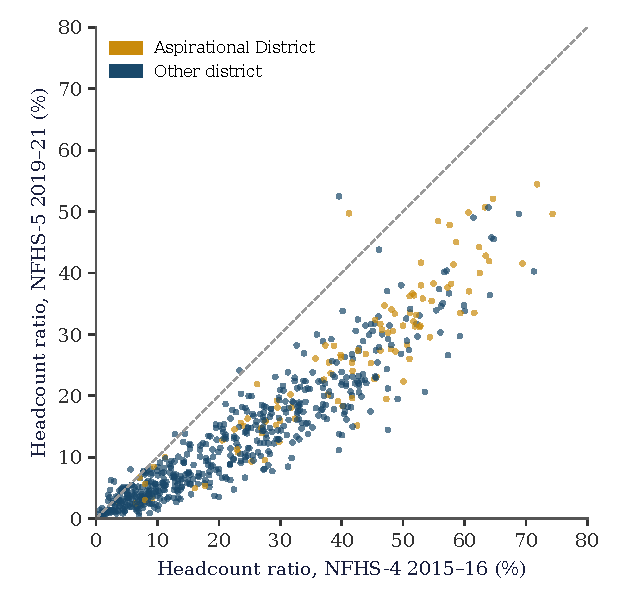
\includegraphics[width=0.55\textwidth]{fig_mpi.pdf}
\caption{District headcount ratio of multidimensional poverty in NFHS-4 and NFHS-5 \citep{niti2023mpi}, for the \hPairN{} districts with comparable estimates in both rounds. Points below the dashed line fell between the two rounds.}\label{fig:mpi}
\end{figure}

\subsection{Poverty and the NFHS indicators}
\Cref{tab:assoc,fig:assoc} relate each of the \nIndAssoc{} NFHS indicators to the NFHS-5 headcount ratio across districts, and also give the median change between rounds for districts with both values. Nine indicators (marked \textdagger) measure an ingredient of the MPI itself---child stunting and underweight, women's low body-mass index, four or more antenatal visits, skilled birth attendance, drinking water, sanitation, electricity and cooking fuel \citep{niti2023mpi}---so part of their association with the headcount ratio is built in; their $|\rho|$ ranges from \rhoCompMin{} to \rhoCompMax. Among indicators that are not MPI ingredients, the strongest associations are with \otherTopOne{} ($\rho = \otherTopOneRho$), \otherTopTwo{} ($\rho = \otherTopTwoRho$) and \otherTopThree{} ($\rho = \otherTopThreeRho$). Of the non-ingredient indicators, \nWeak{} have $|\rho| < 0.2$.

These are correlations between district averages. They describe districts, not individuals \citep{robinson1950}, they are not adjusted for any other factor, and districts are not independent of each other (for example, districts in the same State share policies). They show where indicators move together, not why.

\begin{figure}[!htbp]
\centering
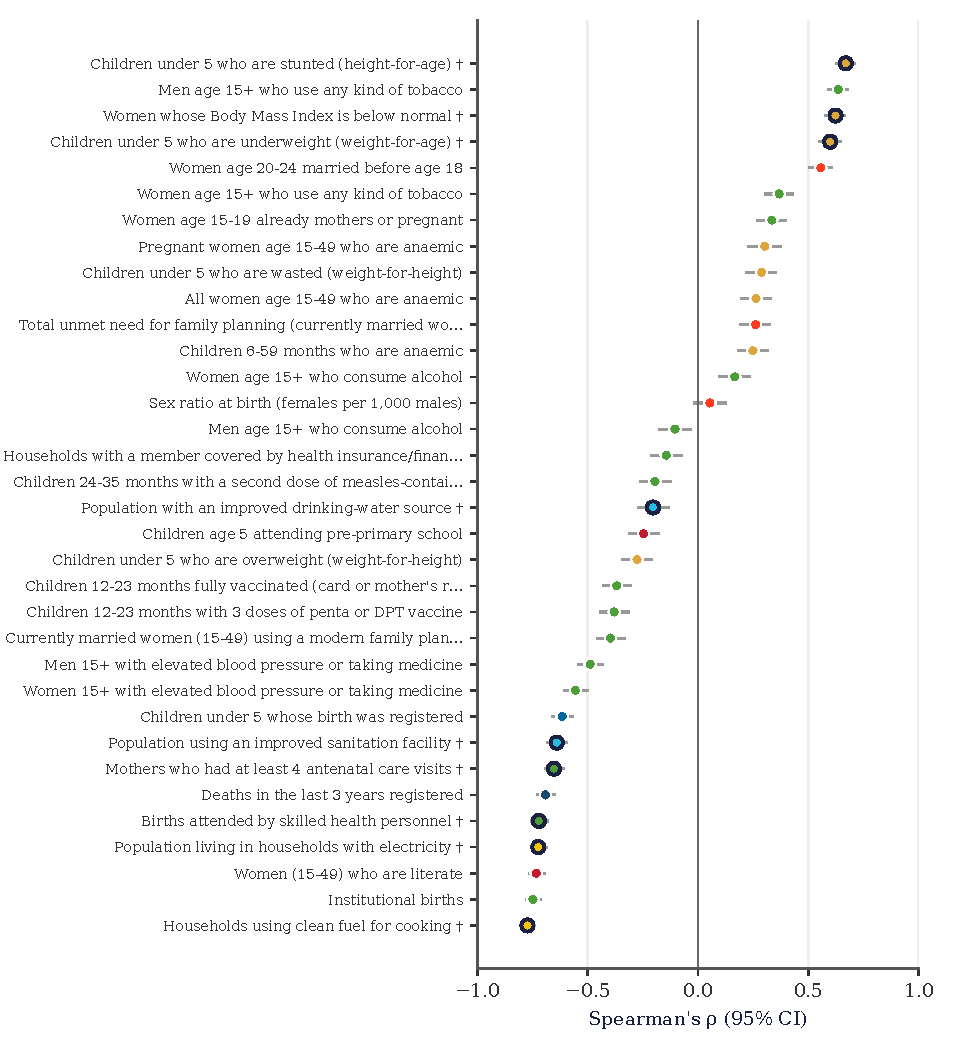
\includegraphics[width=0.95\textwidth]{fig_assoc.pdf}
\caption{Spearman's rank correlation between each NFHS-5 district indicator and the NFHS-5 multidimensional poverty headcount ratio, with 95\% confidence intervals. Colours are the SDG goal colours; outlined points and \textdagger{} mark indicators that are ingredients of the MPI.}\label{fig:assoc}
\end{figure}

{\small
\setlength{\tabcolsep}{4pt}
\begin{longtable}{r>{\raggedright\arraybackslash}p{4.9cm}rrrcc}
\caption{District indicators: number of districts with an NFHS-5 value, median NFHS-5 value, districts with both rounds, median change NFHS-4 to NFHS-5 in percentage points (sex ratio: females per 1{,}000 males) [interquartile range], and Spearman's $\rho$ with the NFHS-5 MPI headcount ratio [95\% CI]. Values are percentages except sex ratio at birth (females per 1{,}000 males). \textdagger{} Ingredient of the MPI.}\label{tab:assoc}\\
\toprule
Goal & Indicator & $n_5$ & Median & $n_{4,5}$ & Change [IQR] & $\rho$ [95\% CI] \\
\midrule
\endfirsthead
\toprule
Goal & Indicator & $n_5$ & Median & $n_{4,5}$ & Change [IQR] & $\rho$ [95\% CI] \\
\midrule
\endhead
\bottomrule
\endfoot
\inputtab{tab_assoc.tex}
\end{longtable}
}

% =====================================================================
\section{The website}\label{sec:web}

The website (\url{https://sahiljangra12.github.io/sdg-explorer-india/}) is a static page served by GitHub Pages that reads only the JSON files written by the pipeline; it computes no new values except the poverty groups, rank correlations and medians described above, each of which is labelled on the page. It has six sections.
\begin{itemize}
  \item \textbf{Home}: the 17 goals in the official SDG colours, each with its number of series and the share of UN series with India data.
  \item \textbf{Goal pages}: one card per series showing India's latest published value. Opening a card shows every value as a table, with breakdowns as columns; a trend chart is offered only when at least three years have values, and chart lines join consecutive years only, so a gap in the data appears as a gap. Published confidence bounds are drawn where available.
  \item \textbf{States and UTs}: the SDG India Index map and ranking, labelled as a composite index.
  \item \textbf{Compare districts}: filters for State, poverty group and Aspirational status; the spread of an indicator across districts; a scatter of the indicator against the poverty headcount ratio with Spearman's $\rho$ (shown only for at least 10 districts) and a warning when the indicator is an MPI ingredient; box plots by group; and a side-by-side profile of up to four districts against the range of all districts.
  \item \textbf{Data gaps}: for each goal, the UN series with and without India data, a series-by-year grid, and the lists of tables and rows not parsed.
  \item \textbf{Sources}: the source register, validation report, data rules and downloads of all processed tables.
\end{itemize}

% =====================================================================
\section{Limitations}\label{sec:limits}

\begin{itemize}
  \item \textbf{State and UT indicator values} are not yet included: the SDG India Index report is a scanned image of low resolution, and the NFHS-5 State compendium files were not reachable from the build machine. Only the published composite scores are used at State level.
  \item \textbf{District context} is limited to poverty and Aspirational status. Census 2011 population, area and urbanisation could not be added because the Census of India website could not be reached from the build environment; district income estimates are produced by individual States with differing methods and years and are not available in one official release for all districts.
  \item \textbf{NFHS files} were obtained from a public mirror; their checksums have not yet been compared with copies from the official site. Chandigarh and Lakshadweep are absent from the fact-sheet set used.
  \item \textbf{Survey uncertainty.} District estimates from NFHS, and the MPI built from them, are sample estimates whose standard errors are not published in the district fact sheets or MPI tables; values in brackets rest on 25--49 cases.
  \item \textbf{Comparability.} NFHS-4 and NFHS-5 districts differ where districts were created in between; the NITI index changed its indicator set between editions; and MoSPI and UN series with the same code are different indicators.
  \item \textbf{Analyses} are unweighted, district-level and descriptive.
\end{itemize}

% =====================================================================
\section{Conclusion}

SDG Explorer India brings India's official SDG data from four publishers into one verified, traceable dataset and makes both the values and the gaps visible. The most consistent finding is how much is missing: fewer than half of the series in the UN global list have any value for India, and nearly a quarter of national series have values for fewer than three years. At district level, NITI Aayog's estimates show multidimensional poverty falling in almost every district with comparable data, and poverty is closely associated with indicators of institutional delivery, women's literacy and civil registration. Adding State-level indicator values, official Census district attributes and published sampling errors are the main next steps.

\section*{Data and code availability}
All code, processed data, verified extracts, provenance records and the website are available at \url{https://github.com/sahiljangra12/sdg-explorer-india} under the MIT License \citep{sdgexplorer}. The underlying data remain subject to each publisher's terms of use; the DataMeet boundaries and the independent NFHS-5 digitisation are licensed CC BY 4.0. The script that generates every number, table and figure in this paper is distributed with it. The project follows the FAIR principles \citep{wilkinson2016fair} as far as a static repository allows.

\section*{Acknowledgements}
The author thanks the United Nations Statistics Division, the Ministry of Statistics and Programme Implementation, NITI Aayog, the Ministry of Health and Family Welfare and the International Institute for Population Sciences for publishing the data, and the DataMeet community and P.~Vardhan for openly licensed resources.

\section*{Use of AI tools}
Software development, data verification scripts and the drafting of this paper were assisted by an AI system (Claude, Anthropic). The author reviewed the code, data and text and is responsible for the content.

\FloatBarrier
\bibliographystyle{plainnat}
\bibliography{references}

\end{document}
